\documentclass[12pt,a4paper,twoside]{scrartcl}
\usepackage[latin1]{inputenc}
\usepackage{amsmath}
\usepackage{amsfonts}
\usepackage{amssymb}
\usepackage{graphicx}
\graphicspath{{images/}}
\usepackage{wrapfig}
\usepackage{fancyhdr}
\usepackage{lastpage}

\date{}
\linespread{1.5}
\pagestyle{fancy}
\fancyhf{}
\fancyhead[LO]{\today}
\fancyhead[CO]{[Filthy Cell-Culture Dish]}
\fancyfoot[R]{Page \thepage\ of \pageref{LastPage}}
\renewcommand{\headrulewidth}{0pt}% disable the underline of the header part


%\setheadsepline{.4pt}
%\setfootsepline{.4pt}
\usepackage[bookmarks=true]{hyperref}
\usepackage{bookmark}
\begin{document}
\begin{center}
\thispagestyle{empty}
\vfill
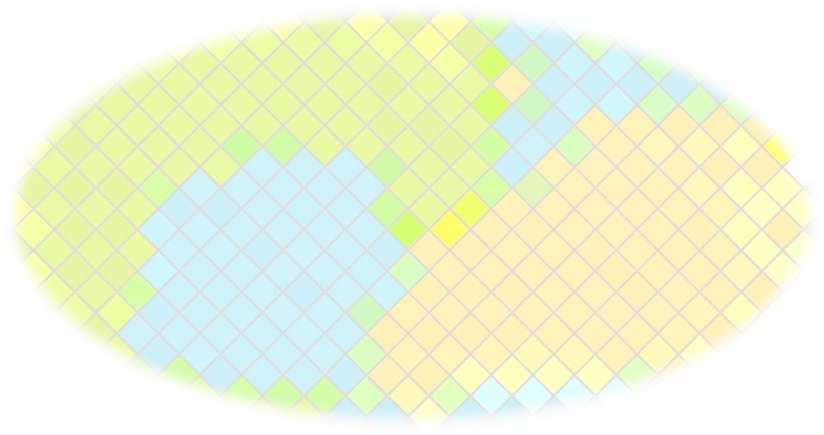
\includegraphics[scale=1]{title2}
\vfill
\huge
	\textbf{Filthy Cell-Culture Dish\\
	User Manuel\\}
\vfill
\large
	(c) YYL Team\\
	Based on Version 1.0.0
\vfill
\end{center}

\clearpage

\large
\textbf{Project Team}
\begin{itemize}
	\item Boyuan Yuan
	\begin{flushright}
		Developer\\
		Storyteller\\
		Graphic Designer\\
		Artwork\\
	\end{flushright}
	
	\item Chunchuan Lv
	\begin{flushright}	
		Developer\\
		Tester\\
		Graphic\\
		Debugger\\
	\end{flushright}
	
	\item Yue Yu
	\begin{flushright}
		Developer\\
		Documentation\\
		Graphic Designer\\
		Artwork\\
	\end{flushright}
\end{itemize}
\clearpage

\large
\textbf{Recommended Requirements}
\begin{list}{}{}
	\item \textbf{CPU:} 2.0GHz i3 Dual Core or equivalent
	\item \textbf{RAM:} 1 GB
	\item \textbf{OS:} Windows 7 or later, Mac OS X 10.8+, GNU/Linux kernel 2.6.18 or later
	\item \textbf{Video Card:} Yes
	\item \textbf{Sound Card:} Yes
	\item \textbf{Free Disk Space:} 500 MB
\end{list}
\clearpage
% Inhaltsverzeichnis	
\pdfbookmark[1]{\contentsname}{toc}\tableofcontents
\clearpage

\section{Introduction to The Game}

This game is a strategy game. Each player creates and evolves a kind of bacteria in an effort to populate the span of a culture dish in a biological laboratory. The game uses a population model with a complex and realistic set of variables and rules to simulate the evolution and competition of the bacteria. Player will be in charge with macro manage: the evolutionary path of his/her species and micro manage: exploration of the small world. The purpose of the game is to take the species into prosperity.

\section{Game Terms}

\subsection{Cell} 

The world in the game is represented by consecutive cells. Individual cell has properties of current population of species and its' environmental limit. There will be additional statistics available for player for decision making.

\subsection{Turn}

Players take turns when playing. For demonstration

\subsection{Explore}

During every turn, each player can choose a cell to explore by clicking that cell and a population advantage for that player's specie will be added to the cell. Players will be challenged to make decisions under an environment of uncertainty. The exploration element allows player treat the game like GO.

\subsection{Traits}

The traits element will make species asymmetry. Therefore, there might be a rich set of strategies emerge.

\section{How to Play}

\section{Game Over}
Game will be over when the whole world is all filled with bacteria. During the competition process, the players can gain a touch of biological knowledge and skills about bacterial reproduction. Moreover, the players will be able to enjoy themselves and feel satisfied during the competition and, possibly, corporation with each other. Therefore, the player will be offered rich opportunities for getting a sense of achievement, recognition, and satisfaction at the same time.

\end{document}